\chapter{Desarrollo Experimental}
\vspace{-1\baselineskip}El esquema de la Figura \ref{fig:expresumen} ilustra grosso modo el desarrollo experimental del trabajo de investigación. Este capítulo presenta los protocolos principales que se siguieron en los experimentos realizados. Algunas metodologías adicionales se incluyeron en las secciones anexas.\enlargethispage{3\baselineskip}
{\floatstyle{boxed}
\restylefloat{figure}
\begin{figure}[H]
    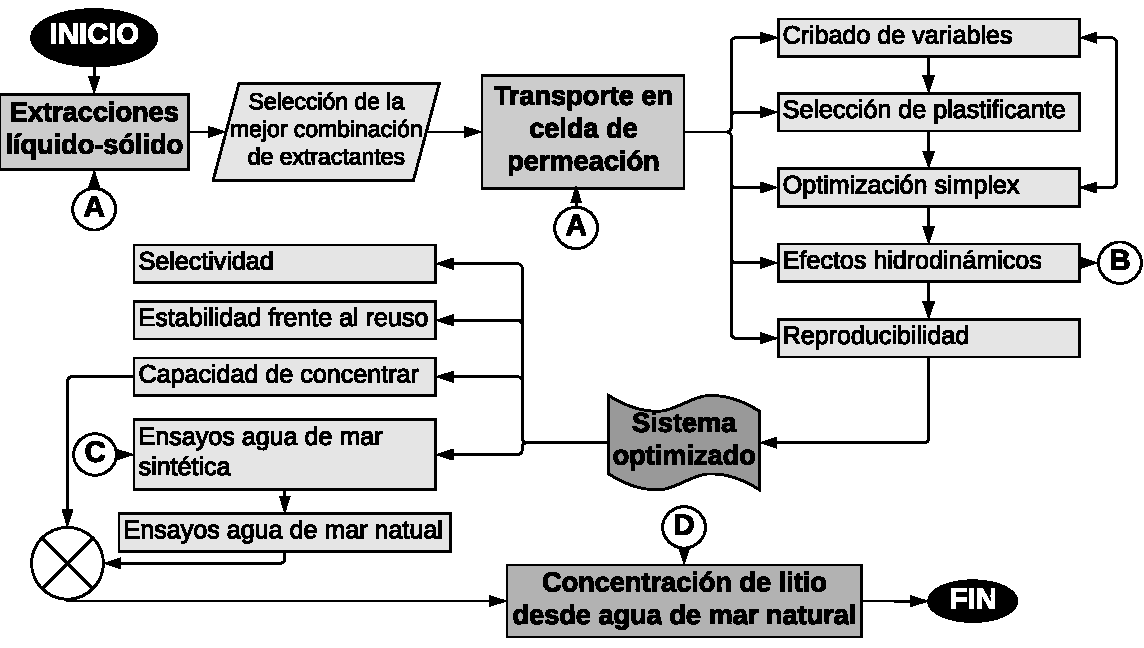
\includegraphics[width=\textwidth]{chap3/summary.pdf}
    \caption[Resumen esquematizado del desarrollo experimental.]{Resumen esquematizado del desarrollo experimental. (A): Determinación de cationes metálicos, (B): Medición de velocidad de giro de las propelas, (C): Precipitación de calcio y magnesio, (D): Microtitulación ácido-base.}
    \label{fig:expresumen}
\end{figure}}

\clearpage\section{Reactivos y disoluciones}
Todas las disoluciones acuosas fueron preparadas usando agua desionizada y reactivos grado analítico. Los proveedores de los extractantes y plastificantes utilizados para la preparación de las membranas se muestran en la Tabla \ref{tab:extractants}. El \ac{CTA} (Aldrich) empleado como polímero base tiene, según el proveedor, un contenido de grupos acetilo de 43.6\% en masa y una masa molecular (promedio en masa) entre 72000 y 74000~g~mol\mnn. 

\begin{table}[H]
    \centering\footnotesize
    \begin{tabular}{@{}p{0.05cm}p{3.5cm}p{5cm}@{}}\toprule
        &\textbf{Nombre}&\textbf{Proveedor}\\\midrule
        \multicolumn{2}{@{}l}{\textit{Extractantes}}\\[-0.6ex]
         & LIX-54-100 (246.0)& Cognis Corporation\\
         & D2EHPA (322.4)& Sigma Aldrich\\
         & TEHP (434.6)& Sigma Aldrich\\
         & Cyanex~923 (348.0) & Cytec Canada Inc.\\
         & TBP (266.3)  & Sigma Aldrich\\
        \multicolumn{2}{@{}l}{\textit{Plastificantes}}\\[-0.6ex]
         & NPOE & Sigma Aldrich\\
         & T2EHP & Sigma Aldrich\\
         & TBEP  & Fluka\\\bottomrule
    \end{tabular}
    \caption[Extractantes y plastificantes empleados.]{Extractantes y plastificantes empleados. En paréntesis se indica la masa molecular de cada extractante en g~mol\mnn.}
    \label{tab:extractants}
\end{table}


Los reactivos diclorometano (\acs{DCM}) \acused{DCM} (J.T. Baker), cloruro de sodio (Químicos Monterey), cloruro de potasio (Merck), cloruro de calcio dihidratado (Merck), sulfato de magnesio heptahidratado (Merck), ácido clorhídrico (Sigma-Aldrich), hidróxido de amonio (Sigma-Aldrich), fosfato monohidrógeno de amonio (Merk) e hidróxido de sodio (Mallinckrodt) se usaron tal y como fueron recibidos. Disoluciones de cloruro de litio y cloruro de magnesio fueron preparadas di\-sol\-vien\-do sus respectivos carbonatos (Aldrich) en un ligero exceso de ácido clorhídrico.

Todas las disoluciones y sus subsecuentes diluciones fueron preparadas gravimétricamente en una balanza analítica OHAUS Adventurer AX224. Esta práctica concede una gran versatilidad para hacer las disoluciones y permite el manejo de cantidades de disolución muy pequeñas, sin sacrificar precisión en la toma de la alícuota. Adicionalmente, preparar las disoluciones en masa permite un uso más eficiente del material de laboratorio y del tiempo del experimentador.

Cuando se indica que un reactivo se usó {seco}, se hace alusión a que la posible humedad presente en dicho reactivo fue retirada usando un horno de convección forzada a una temperatura de 80$^o$C durante una hora y el reactivo se dejó enfriar en un desecador donde permaneció hasta el momento de su uso.

La cuantificación de cationes metálicos se hizó por espectrometría de absorción atómica por llama (\acs{FAAS})\acused{FAAS} y espectrometría de emisión atómica por llama (\acs{FAES})\acused{FAES}, en un espectrómetro de absorción atómica Perkin-Elmer 3100, usando las configuraciones recomendadas por el fabricante \citep{perkin}. Los detalles del sistema analítico se describen en el Anexo \ref{sec:quantification}.

El protocolo de lavado del material de laboratorio implicó tres etapas principales:
\begin{enumerate}
    \item Lixiviación de especies metálicas por inmersión en ácido nítrico al 10\% en volumen durante al menos 12 horas.
    \item Enjuague vigoroso con agua desionizada al menos tres veces.
    \item Secado en horno de convección forzada a una temperatura entre 60 y 80$^o$C y enfriamiento a temperatura ambiente.
\end{enumerate}


\subsection{Agua de mar sintética}\index{Agua de mar!sintética}
El agua de mar sintética fue preparada acorde a una receta simplificada de agua de mar que se usa en la determinación de constantes termodinámicas en agua de mar \citep{Sun2019}. La composición se muestra en la Tabla \ref{tab:seasintetic} \citep{Dickson1994}. En esta receta se consideran únicamente las especies cuya concentración es relativamente alta. Se incluyen los aniones cloruro y sulfato mientras los aniones bromuro y fluoruro son reemplazados por cloruro y los demás aniones son ignorados. El catión estroncio es reemplazado por calcio, el cual es considerado en conjunto con sodio, potasio y magnesio. El ion litio no se incluye en la receta simplificada pero se añadió a la concentración promedio reportada para agua de mar: 0.18~mg~kg\mnn\ (2.6\e{-5}~mol~kg\mnn) \citep{Evans2013}. 

La fuerza iónica de la disolución sintética es la misma que la fuerza iónica promedio reportada para el agua de mar real (0.697~mol~kg\mnn).

\begin{table}[H]
    \centering\footnotesize
    \begin{tabular}{@{}p{0.05cm}lld{2.3}c@{}}\toprule
        &\multirow{2}{*}{\textbf{Especie}} & \multicolumn{2}{c}{\textbf{Concentración}}&\textbf{Rel. molar}\\
        &&mol~kg\mnn&\multicolumn{1}{c}{g~kg\mnn}&\multicolumn{1}{c}{\ce{M^n+}:\ce{Li^+}}\\\midrule
        \multicolumn{2}{l}{\textit{Aniones}}\\[-0.6ex]
        &\ce{Cl^-}  &0.549 &19.472&-\\
        &\ce{SO4^2-}&0.028 &2.720 &-\\
        \multicolumn{2}{l}{\textit{Cationes}}\\
        &\ce{Na^+}  &0.469 &10.785&18000\\
        &\ce{Mg^2+} &0.052 &1.284 &2030\\
        &\ce{Ca^2+} &0.010 &0.415 &400\\
        &\ce{K^+}   &0.010 &0.399 &390\\
        &\ce{Li^+}  &2.6\e{-5}&\multicolumn{1}{c}{1.8\e{-4}}&1\\\bottomrule
    \end{tabular}
    \caption{Composición del agua de mar sintética simplificada.}
    \label{tab:seasintetic}
\end{table}

\subsection{Muestras de agua de mar natural}\index{Agua de mar!natural}
Dos muestras de agua de mar natural fueron recolectadas manualmente en cercanías a las playas de Santa Marta-Colombia y de St. George Island-Estados Unidos (Figura \ref{fig:SWNmap}). En cada punto se recolectó cerca de un litro de agua de mar en botellas de poli(tereftalato de etileno) (PET)\acused{PET}, y las muestras fueron mantenidas bajo refrigeración hasta su uso. Previo a su uso, las muestras se filtraron por gravedad para remover arena y otros sólidos. Los puntos de recolección de las muestras fueron escogidos por la disponibilidad de las personas que se encargaron de hacer el muestreo.

\begin{figure}[htbp]
    \centering
    \subbottom{\begin{picture}(500,300)
               \put(0, 0){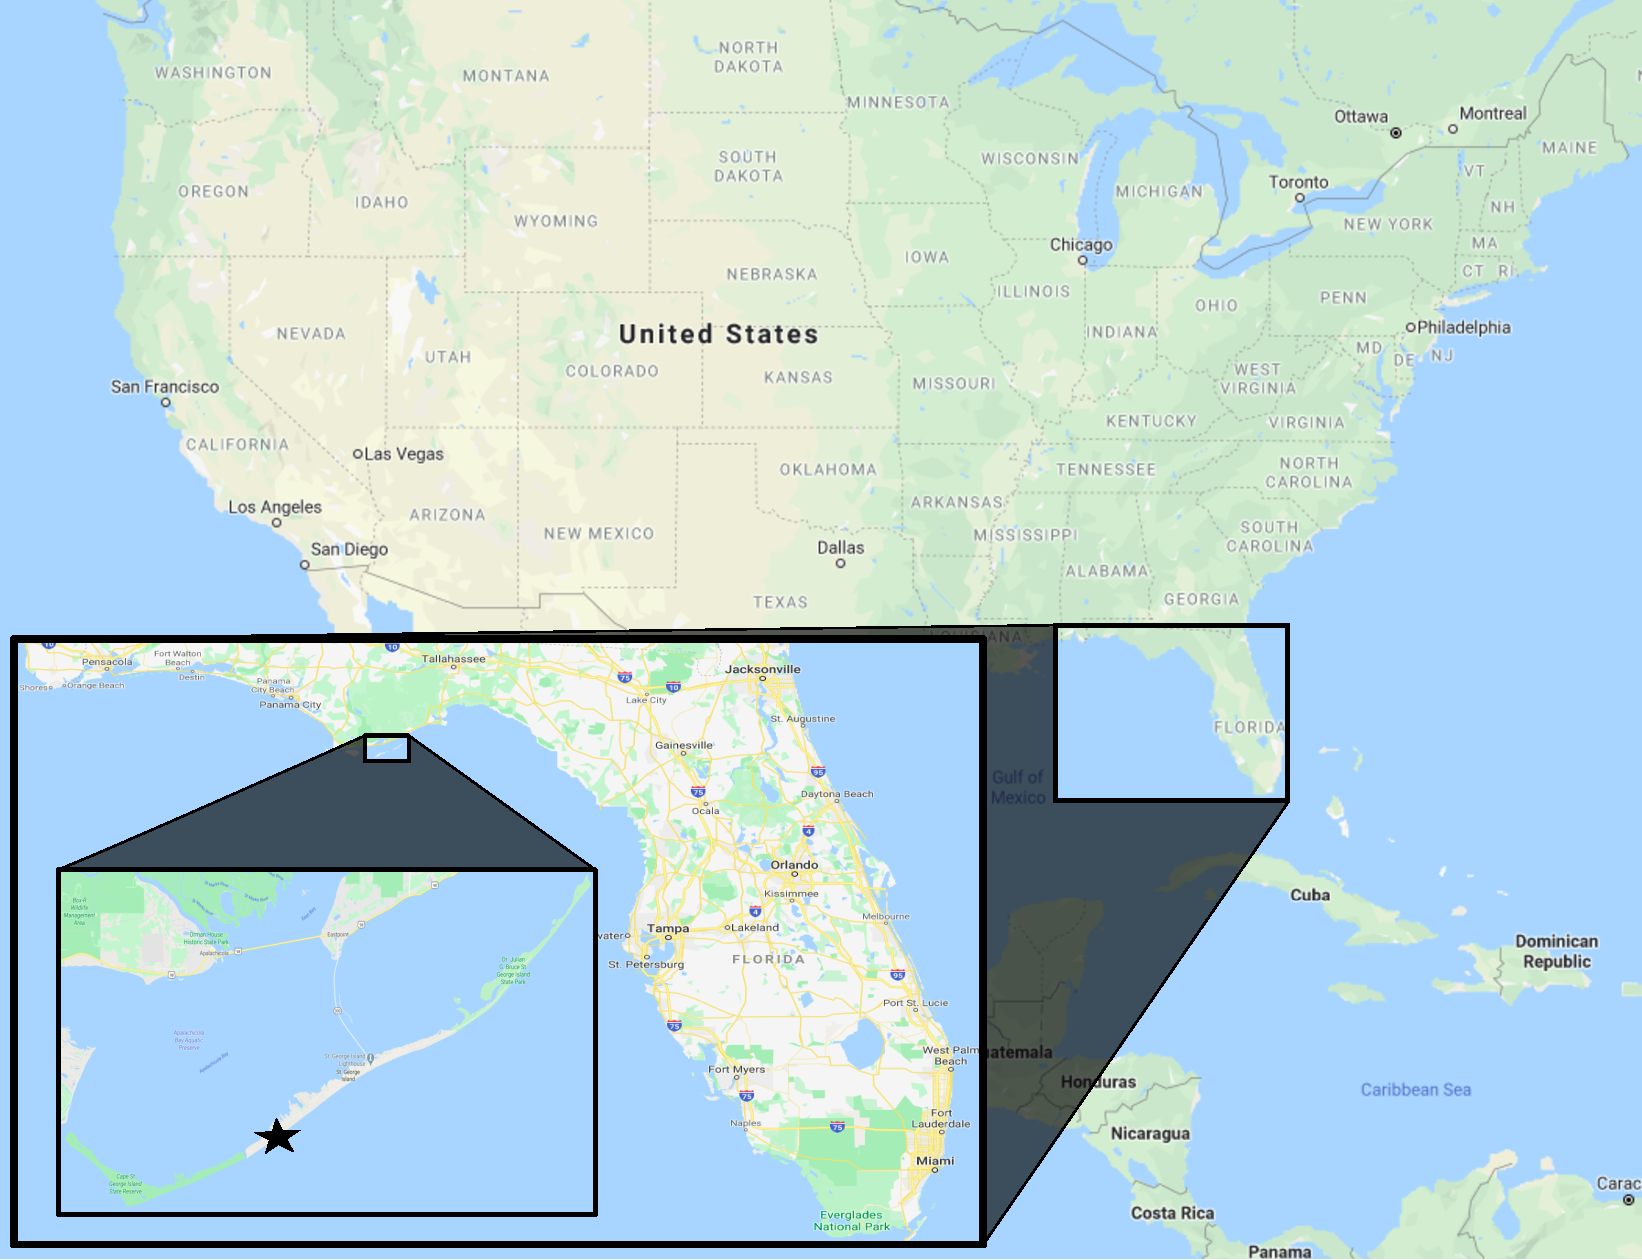
\includegraphics[width=\textwidth,trim={0 0 0 4cm}, clip]{chap3/SWN.pdf}}
               \put(3, 278){\Large a)}
               \end{picture}}\\%
    \subbottom{\begin{picture}(550,300)
               \put(0, 0){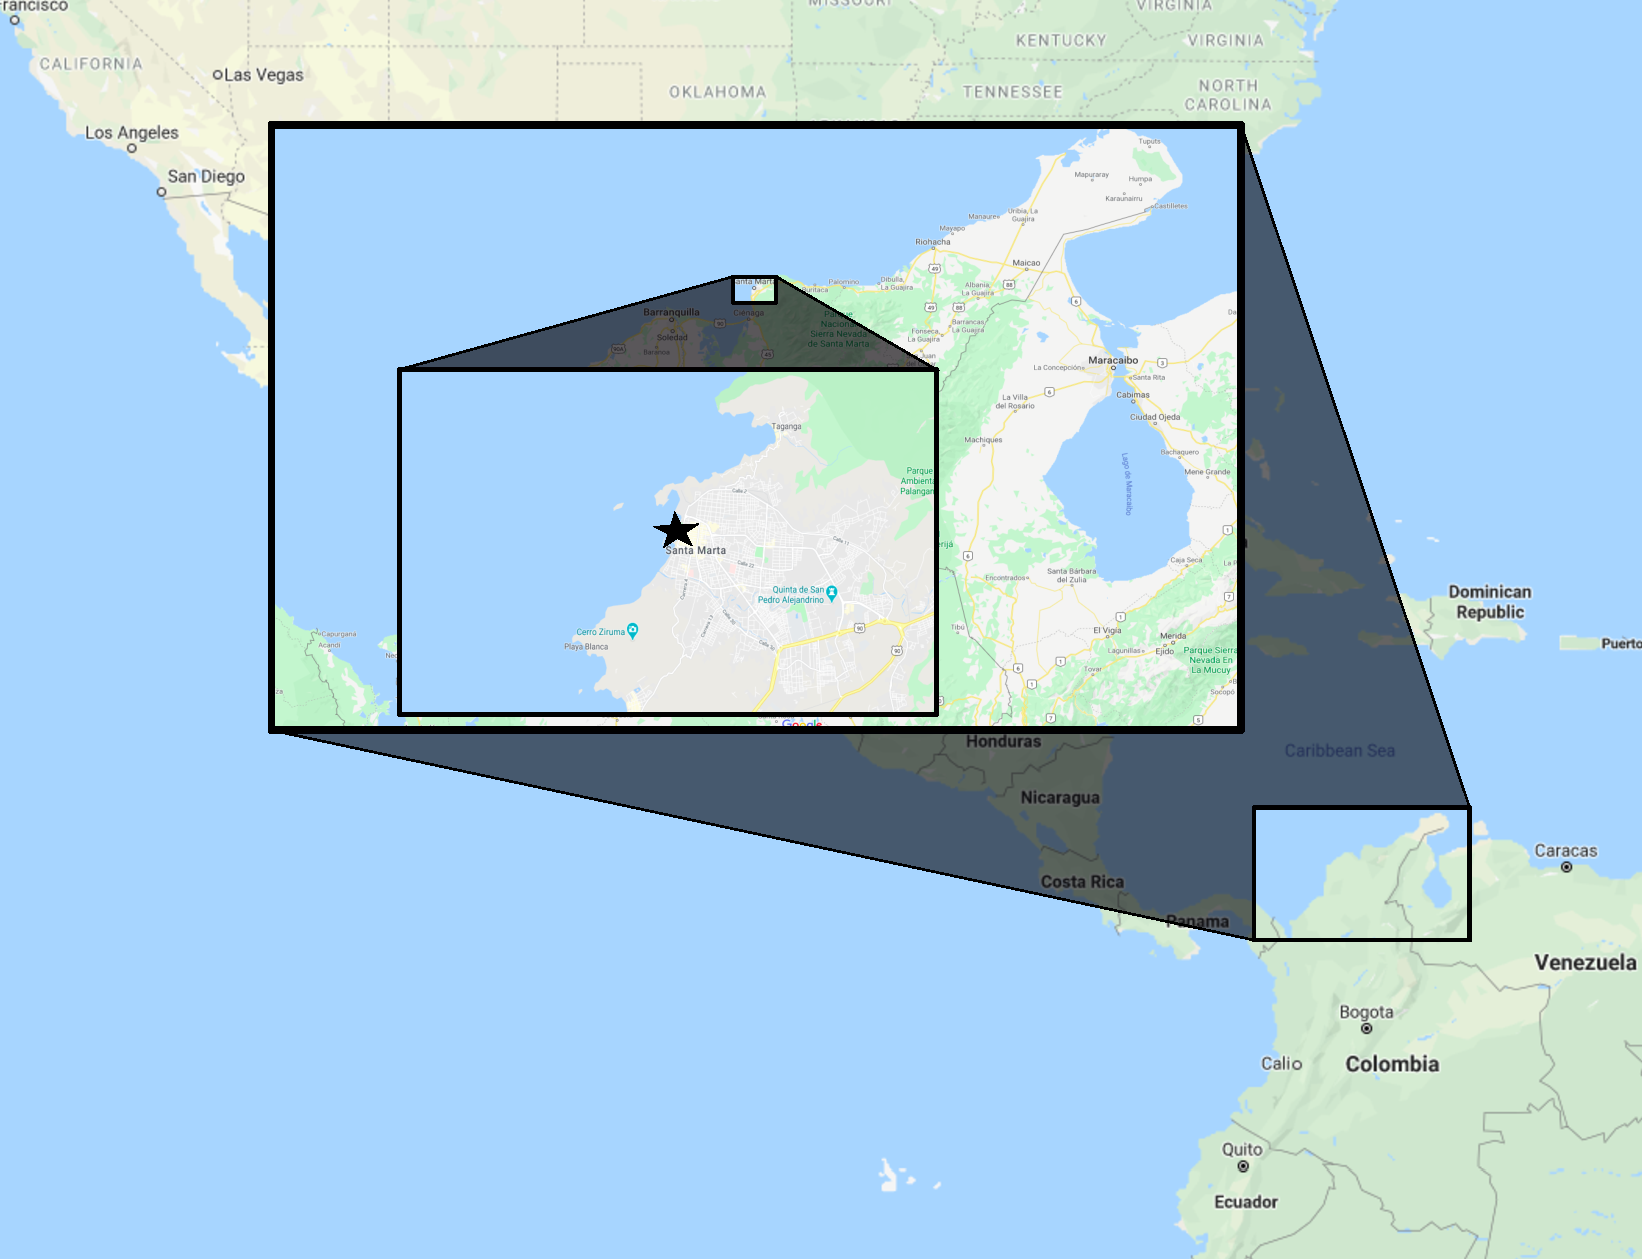
\includegraphics[width=\textwidth,trim={0cm 2.5cm 0cm 1.5cm}, clip]{chap3/SWS.pdf}}
               \put(3, 278){\Large b)}
               \end{picture}}
    \caption[Ubicación geográfica de los puntos de muestreo de agua de mar.]{Ubicación en  Estados Unidos (a) y en Colombia (b) de los puntos de muestreo (\protect\starfvpointsblck) de agua de mar natural.}
    \label{fig:SWNmap}
\end{figure}

\section{Elaboración de membranas poliméricas de inclusión}\index{PIM!elaboración}
Las membranas fueron preparadas por el método de vertido en molde descrito por varios autores \citep{Salazar-alvarez2005}. En un vaso de precipitados de 10~mL se toman cuidadosamente las masas escogidas de polímero base (\ac{CTA}), extractantes, y plastificante (la mayoría de las membranas no necesitaron plastificante en su formulación). Se añaden 10~mL de \ac{DCM} y la mezcla se agita magnéticamente durante aproximadamente dos horas hasta que se observa la disolución completa del polímero base. La disolución homogénea se transfiere cuantitativamente a la sección inferior de una caja Petri de vidrio (Pyrex\textregistered) y se cubre con su tapa respectiva. El disolvente se deja evaporar lentamente durante toda la noche en una campana de extracción sin encender. Se forman películas homogéneas que por lo general son flexibles y poseen buenas propiedades mecánicas. Las membranas pueden dejarse en las cajas de Petri por un periodo largo de tiempo sin que sufran un deterioro importante en su desempeño. 

Para retirar las membranas al momento de su uso se inunda la caja de Petri con agua desionizada y se corta el borde de la membrana que colinda con la pared circular del recipiente, usando la punta redonda de una microespátula delgada de acero inoxidable. Con estos dos pasos la membrana puede despegarse con facilidad, y el riesgo de que se dañe en este proceso disminuye considerablemente.

El grosor de las membranas se determinó usando un micrómetro digital de tornillo (Fowler IP54). La medición de grosor conlleva un deterioro a la membrana que impide su uso posterior para experimentos de transporte por lo que estas membranas ya no pueden usarse para nada más. Para medir el grosor, se dibuja una cuadrícula sobre la membrana usando un rotulador permanente de punta fina y se determina el grosor en cada cuadrado que tiene aproximadamente 0.5~cm de lado. Los valores que corresponden al centro con 1.25~cm a la redonda (región que está en contacto con las disoluciones) son promediados y el promedio es el valor que se reporta.

\section{Extracción líquido-sólido}\label{sec:liqsolex}\index{Extracción!líquido-sólido}
Las extracciones líquido-sólido se hicieron para seleccionar la combinación de extractantes con los que se trabajaría durante todo el proyecto. Se usó un agitador mecánico Burrell Scientific Wrist Action$^{TM}$ Modelo 75 cargado con tubos cónicos de 50~mL con tapa rosca (tubos de centrífuga). Para la extracción, se dispuso en el tubo una masa conocida de una disolución alcalina con ion litio (fase donadora) y una \ac{PIM}. Para maximizar el área de contacto de la disolución con la membrana, se procuró que ésta quedara suspendida en la disolución y no en contacto con la pared interior del tubo. La mezcla se agitó vigorosamente durante tres horas, al cabo de las cuales la membrana se extrajo con pinzas y se lavó cuidadosamente con agua desionizada. Posteriormente, la recuperación del ion litio extraído por la membrana se hizo con un protocolo similar usando una disolución de ácido clorhídrico (fase receptora). La concentración de ion litio en la fase donadora y receptora se determinó antes y después de cada proceso de agitación.

\section{Transporte en celda de permeación}
Los experimentos de transporte se hicieron en una celda de permeación (o celda de transporte) similar a la ilustrada en la Figura \ref{fig:celda}. La celda consta de dos compartimientos separables (semiceldas) que se encuentran conectados a través de un orificio circular de 2.5~cm de diámetro. En cada semicelda se disponen las disoluciones de alimentación y de recuperación, respectivamente. El orificio circular sirve para posicionar la membrana que queda firmemente sujetada entre las semiceldas que se mantienen juntas con firmeza, gracias al uso de pinzas clip metálicas para papel de 5~cm. El sello entre los compartimientos se logra con un empaque circular tipo \textit{o-ring}.

\begin{figure}[H]
    \centering
    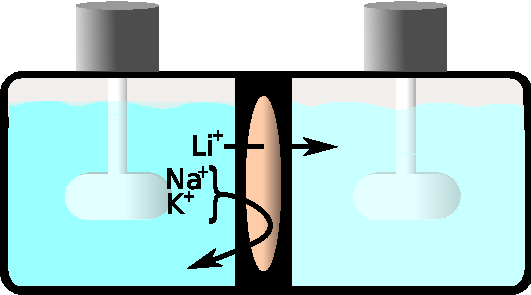
\includegraphics[width=0.5\textwidth]{chap3/PermCell}
    \caption{Celda de permeación usada en los experimentos de transporte.}
    \label{fig:celda}
\end{figure}

Las semiceldas son agitadas mecánicamente con propelas de doble aspa de teflón, impulsadas por motores eléctricos controlados individualmente por moduladores de amplitud de pulso (\acs{PWM})\acused{PWM}. Por lo general se inicia con 85~g de disolución en cada compartimiento y periódicamente se toman pequeñas alícuotas (entre 800 y 1500~$\mu$L) de ambas disoluciones. Las alícuotas son almacenadas en viales Eppendorf\textregistered~ para cuantificar posteriormente las especies de interés (Anexo \ref{sec:quantification}).

Las condiciones del proceso de transporte (composición de las membranas y de las disoluciones de alimentación y recuperación) fueron optimizadas por medio de diseños experimentales factoriales fraccionados y del algoritmo simplex modificado. Para esto se usaron los paquetes de R \verb|FrF2| de \cite{FrF2} y \verb|labsimplex| de \cite{labsimplex}. Los detalles de las matrices de diseño o de la configuración inicial del simplex se incluyen en la sección de resultados.

\subsection{Efecto de las condiciones hidrodinámicas y reproducibilidad}\label{sec:hydroexpe}
Las condiciones hidrodinámicas fueron evaluadas con experimentos de transporte modificando la rapidez de rotación de la propela ($\Theta$) que agita cada disolución. Esta rapidez de rotación se determinó siguiendo el protocolo descrito en el Anexo \ref{App:tracker}. Inicialmente se evaluaron valores de $\Theta$ entre 360 y 920 revoluciones por minuto (\ac{RPM}\acused{RPM}) mientras la rapidez de agitación en la fase de recuperación se mantuvo constante en $960\pm60$~\ac{RPM}. Cada proceso de transporte fue monitoreado durante 5 horas y se usaron disoluciones de alimentación de ion litio en ausencia de interferentes.

Posteriormente, para evaluar la repoducibilidad del proceso, el transporte se llevó a cabo en días distintos, en un intervalo de valores de rapidez de agitación más pequeño (510 a 665 \ac{RPM}). Se usó como variable de bloqueo la celda en la que se llevó a cabo el transporte (Celda A y Celda B) y se usaron disoluciones de alimentación con ion litio en presencia de un exceso molar 1:20 de iones sodio. La concentración de ambas especies fue monitoreada durante cinco horas.

\subsection{Selectividad frente a sodio, potasio y magnesio}\index{PIM!selectividad}
La selectividad del sistema optimizado frente a los iones sodio, potasio y magnesio (cationes interferentes) se estudió por medio de transportes usando disoluciones de alimentación con ion litio 2~mg~kg\mnn\ en presencia de cada uno de los cationes interferentes en relaciones molares \ce{Li+}/\ce{M^n+} de 1:1, 1:10 y 1:100. Se usó una disolución de alimentación con concentración inicial de hidróxi\-do de amonio de 0.016~mol~kg\mnn\ y una disolución de recuperación de ácido clorhídrico a una concentración inicial de 0.10~mol~kg\mnn. Cada proceso de transporte fue monitoreado durante 5 horas.

\subsection{Capacidad de reuso de la membrana}\label{sec:reuseex}\index{PIM!estabilidad}
La capacidad de reuso de la membrana se estudió repitiendo el proceso de transporte renovando las disoluciones de alimentación y de recuperación. El ciclo se llevó a cabo 10 veces consecutivas usando la misma membrana optimizada y una disolución de alimentación ideal (hidróxido de amonio 0.016~mol~kg\mnn\ y ion litio 2~mg~kg\mnn) en la que el ion litio era el único catión metálico presente (proveniente de cloruro de litio). Se usó ácido clorhídrico 0.10~mol~kg\mnn\ como disolución de recuperación.

\subsection{Concentración de ion litio}\label{ss:concentracion}
Los experimentos de concentración fueron similares a los descritos en la Sección \ref{sec:reuseex}, con la diferencia de que la disolución de recuperación no se renovó entre ciclos con el fin de concentrar el ion litio en esta fase. Adicionalmente el número de ciclos consecutivos fue menor. En primera instancia, se utilizo la misma disolución de alimentación ideal de la sección anterior y esta fue renovada cuatro veces (cinco ciclos). Posteriormente, luego de comprobar que el sistema era capaz de extraer ion litio de agua de mar sintética y natural (Sección \ref{sec:resultsSSS}), se usó agua de mar natural a partir de la cual se extrajo el ion litio durante cuatro ciclos. 

Para concentrar ion litio desde agua de mar fue necesario restaurar la concentración de iones hidronio en la disolución de alimentación al final de cada ciclo usando ácido clorhídrico 1~mol~kg\mnn. No se mantuvo constante la acidez de la disolución de recuperación porque se quiso evitar el uso de sustancias amortiguadoras de pH que representarían variables adicionales que considerar al momento de optimizar el sistema. La cantidad de ácido necesaria para ajustar nuevamente la concentración de iones hidronio al valor deseado fue estimada considerando la concentración de ácido remanente, la cual fue determinada por microtitulación con hidróxido de sodio (Anexo \ref{Sec:microfuck}).

\subsection{Extracción de ion litio de agua de mar}\index{Agua de mar}
Para extraer ion litio de agua de mar fue necesario separar del medio los cationes divalentes calcio y magnesio antes del proceso de transporte (Sección \ref{sec:selecresults}). La manera más sencilla y eficiente de hacerlo es por precipitación como se describe en el siguiente apartado. Como resultado de una de las etapas de precipitación, la disolución de alimentación queda con un exceso de iones hidroxilo que provee a la disolución de un medio lo suficientemente alcalino como para favorecer el transporte de iones litio hacia la fase de recuperación. Debido a esto, no fue necesaria la adición de hidróxido de amonio para el proceso de transporte.

%En los ensayos con agua de mar natural, la concentración en exceso de iones hidroxilo fue determinada por microtitulación ácido-base y se estudió el efecto de su valor inicial en el transporte de litio a través de la membrana. Para esto, distintas proporciones de los iones hidroxilos en exceso fueron neutralizados con ácido clorhídrico 1~mol~kg\mnn\ a concentraciones iniciales de hidróxido de 0.04, 0.03, 0.02, 0.01 y 0.00~mol~kg\mnn.
 
\subsubsection{Eliminación de cationes divalentes calcio y magnesio}\label{sec:preci}
Los iones calcio y magnesio fueron eliminados de las matrices de agua de mar sintética y agua de mar natural por precipitación en dos pasos. En primera instancia, el magnesio es removido como hidróxido usando hidróxido de sodio a una concentración de 0.15 mol~kg\mnn. Esto aumenta apreciablemente la cantidad de iones sodio presente en la muestra. Una porción de los iones calcio coprecipitan con el magnesio como hidróxido. En un segundo paso, los iones calcio remanentes son removidos como fosfatos al añadir fosfato monohidrógeno de amonio a una concentración 0.005~mol~kg\mnn. 

Tras la adición de cada reactivo precipitante, la mezcla es agitada vigorosamente por cinco mi\-nu\-tos y posteriormente se separan las fases por centrifugación a 3000 \ac{RPM} durante cinco minutos (IEC HN-SII Centrifuge, Damon/IEC Division).

\clearpage\ChapBib{chap3/experimental}